% SC4242 --- Chapter 1: Compiler Overview & Phases (0->100 ground-up)
\chapter{Compiler Overview and Phases}
\label{ch:overview}

\begin{quote}
\emph{``A compiler translates, optimises, and trusts no input.''} --- From characters on a screen to bytes a CPU executes, a compiler bridges two worlds by repeated, well-defined transformations.
\end{quote}

\noindent\fbox{\parbox{\dimexpr\linewidth-2\fboxsep-2\fboxrule}{%
\textbf{From zero: we build here, no compiler background needed.} We assume only that a program is text and a computer executes machine code. Every notion---source language, target language, phase, pass, intermediate representation---is defined from scratch with pictures before formalism. No SC2203 or SC1007 is assumed without recap.}}
\vspace{0.4em}

\section*{Learning Outcomes}
After this chapter you will be able to:
\begin{enumerate}[label=(L\arabic*)]
    \item distinguish compiler, interpreter, and hybrid (JIT) execution models;
    \item name and place the six core phases: lexing, parsing, semantic analysis, IR lowering, optimisation, code generation;
    \item explain front-end vs.\ middle-end vs.\ back-end separation and why IR matters;
    \item trace a tiny program \texttt{a = b + c*2} through tokens, tree, IR, and assembly;
    \item reason about pass ordering, diagnostics, and what ``correct compilation'' means.
\end{enumerate}

% ============================================================
\section{Why Compilers? Source, Target, and Trust}
\label{sec:why-compilers}
\emph{Intuition:} you write in a human-friendly language (Python, C, Java); the hardware understands only numbers---opcodes, registers, addresses. A compiler is a total function $\text{compile}: \text{Source} \to \text{Target}$ that must preserve meaning while fitting hardware constraints. If it mistranslates, the bug is invisible at source level.

A \emph{source language} is a set of legal texts defined by a grammar; a \emph{target language} is the instruction set (e.g., ARM, x86, JVM bytecode). The compiler's contract is \emph{semantics preservation}: for every source program $P$, the observable behaviour of $\text{compile}(P)$ equals that of $P$ (modulo undefined behaviour).

We build this contract stepwise. Rather than one giant translation, we pipeline small, testable steps---phases---each with a precise input/output data structure.

\begin{definition}[Phase vs.\ pass]
A \emph{phase} is a logical task (e.g., parsing). A \emph{pass} is a traversal over an intermediate representation (IR). One phase may be one or many passes; one pass may serve multiple phases for efficiency.
\end{definition}

\begin{example}[Interpreter vs.\ compiler vs.\ hybrid]
CPython interprets: loop reads source, executes. GCC compiles ahead-of-time (AOT): source $\to$ object file once. HotSpot JVM is hybrid: interprets first, then JIT-compiles hot methods (Ch.~8). The trade-off is start-up latency vs.\ peak throughput.
\end{example}

% TikZ 1: compiler pipeline conveyor
\begin{figure}[h]
\centering
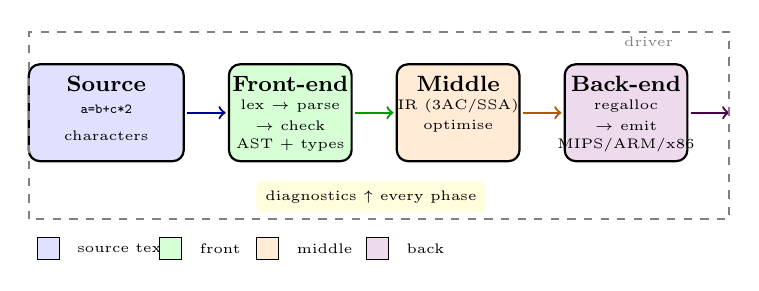
\begin{tikzpicture}[scale=0.82,every node/.style={font=\scriptsize}]
\draw[thick,fill=blue!12,rounded corners=4pt] (0,0) rectangle (2.4,1.5);
\node[font=\footnotesize\bfseries] at (1.2,1.2) {Source};
\node[font=\tiny] at (1.2,0.8) {\texttt{a=b+c*2}};
\node[font=\tiny] at (1.2,0.4) {characters};
\draw[->,thick,blue!60!black] (2.45,0.75)--(3.05,0.75);
\draw[thick,fill=green!16,rounded corners=4pt] (3.1,0) rectangle (5.0,1.5);
\node[font=\footnotesize\bfseries] at (4.05,1.2) {Front-end};
\node[font=\tiny] at (4.05,0.85) {lex $\to$ parse};
\node[font=\tiny] at (4.05,0.55) {$\to$ check};
\node[font=\tiny] at (4.05,0.25) {AST + types};
\draw[->,thick,green!60!black] (5.05,0.75)--(5.65,0.75);
\draw[thick,fill=orange!16,rounded corners=4pt] (5.7,0) rectangle (7.6,1.5);
\node[font=\footnotesize\bfseries] at (6.65,1.2) {Middle};
\node[font=\tiny] at (6.65,0.85) {IR (3AC/SSA)};
\node[font=\tiny] at (6.65,0.55) {optimise};
\draw[->,thick,orange!70!black] (7.65,0.75)--(8.25,0.75);
\draw[thick,fill=violet!14,rounded corners=4pt] (8.3,0) rectangle (10.2,1.5);
\node[font=\footnotesize\bfseries] at (9.25,1.2) {Back-end};
\node[font=\tiny] at (9.25,0.85) {regalloc};
\node[font=\tiny] at (9.25,0.55) {$\to$ emit};
\node[font=\tiny] at (9.25,0.25) {MIPS/ARM/x86};
\draw[->,thick,violet!60!black] (10.25,0.75)--(10.85,0.75);
\node[font=\tiny,fill=yellow!14,rounded corners=2pt] at (5.3,-0.55) {diagnostics $\uparrow$ every phase};
\draw[thick,dashed,gray] (0,-0.9) rectangle (10.85,2.0);
\node[font=\tiny,gray] at (9.6,1.85) {driver};
% legend
\node[draw,fill=blue!12,minimum size=0.28cm] at (0.3,-1.35) {};
\node[font=\tiny,anchor=west] at (0.6,-1.35) {source text};
\node[draw,fill=green!16,minimum size=0.28cm] at (2.2,-1.35) {};
\node[font=\tiny,anchor=west] at (2.5,-1.35) {front};
\node[draw,fill=orange!16,minimum size=0.28cm] at (3.7,-1.35) {};
\node[font=\tiny,anchor=west] at (4.0,-1.35) {middle};
\node[draw,fill=violet!14,minimum size=0.28cm] at (5.4,-1.35) {};
\node[font=\tiny,anchor=west] at (5.7,-1.35) {back};
\end{tikzpicture}
\caption{The compiler pipeline: characters $\to$ tokens $\to$ AST $\to$ IR $\to$ optimised IR $\to$ target. The driver orchestrates passes and surfaces diagnostics.}
\label{fig:pipeline}
\end{figure}

% ============================================================
\section{The Six Phases in Detail}
\label{sec:six-phases}
We fix a tiny running language: expressions with $+$, $*$, assignment, integers, and variables.

\paragraph{Lexical analysis (Ch.~2)} groups characters into \emph{tokens}: \texttt{a}, \texttt{=}, \texttt{b}, \texttt{+}, \texttt{c}, \texttt{*}, \texttt{2}. Whitespace and comments are discarded. Output: token stream with source locations.

\paragraph{Syntax analysis / parsing (Ch.~3)} arranges tokens into a tree per a \emph{context-free grammar}. Leaves are tokens; internal nodes are syntactic categories. Output: parse tree $\to$ \emph{abstract syntax tree} (AST) that drops punctuation.

\paragraph{Semantic analysis (Ch.~4)} checks meaning: are names declared? do types align? It maintains a \emph{symbol table} (scopes $\to$ declarations) and annotates the AST with types. Errors here are not syntax errors but ``no such variable'' or ``cannot add string to int''.

\paragraph{Intermediate representation (Ch.~5)} lowers the AST to a simpler, uniform IR such as \emph{three-address code} (3AC) and \emph{SSA}. IR is where most tooling lives: it is target-independent yet close to machine.

\paragraph{Optimisation (Ch.~6)} rewrites IR to preserve semantics while improving time/space/energy. Analyses (dataflow) determine what is safe; transforms apply it.

\paragraph{Code generation (Ch.~7)} maps IR to target instructions, selecting instructions, scheduling them, and allocating registers ($k$ physical from unbounded virtuals).

\begin{definition}[Front / middle / back]
\emph{Front-end} = source-dependent (lex, parse, type-check; $n$ front-ends for $n$ languages). \emph{Back-end} = target-dependent (instruction selection, regalloc; $m$ back-ends for $m$ targets). \emph{Middle-end} = IR + optimisation, shared: $n+m$ work instead of $n\times m$ without IR. This is why LLVM has one IR for many languages/targets.
\end{definition}

% TikZ 2: pass vs phase + front/middle/back Venn
\begin{figure}[h]
\centering
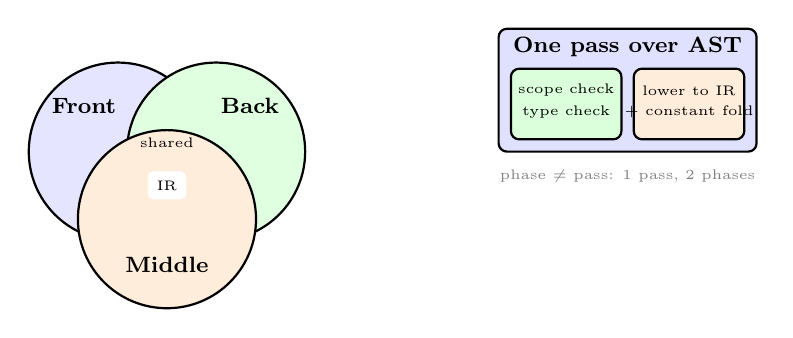
\begin{tikzpicture}[scale=0.78,every node/.style={font=\scriptsize}]
\begin{scope}
\draw[thick,fill=blue!10] (0,0) circle (1.45cm);
\draw[thick,fill=green!12] (1.6,0) circle (1.45cm);
\draw[thick,fill=orange!14] (0.8,-1.1) circle (1.45cm);
\node[font=\footnotesize\bfseries] at (-0.55,0.75) {Front};
\node[font=\footnotesize\bfseries] at (2.15,0.75) {Back};
\node[font=\footnotesize\bfseries] at (0.8,-1.85) {Middle};
\node[font=\tiny,fill=white,rounded corners=2pt] at (0.8,-0.55) {IR};
\node[font=\tiny] at (0.8,0.15) {shared};
\end{scope}
\begin{scope}[xshift=6.2cm]
\draw[thick,fill=blue!12,rounded corners=3pt] (0,0) rectangle (4.2,2.0);
\node[font=\footnotesize\bfseries] at (2.1,1.7) {One pass over AST};
\draw[thick,fill=green!14,rounded corners=3pt] (0.2,0.2) rectangle (2.0,1.35);
\node[font=\tiny] at (1.1,1.0) {scope check};
\node[font=\tiny] at (1.1,0.65) {type check};
\draw[thick,fill=orange!14,rounded corners=3pt] (2.2,0.2) rectangle (4.0,1.35);
\node[font=\tiny] at (3.1,1.0) {lower to IR};
\node[font=\tiny] at (3.1,0.65) {+ constant fold};
\node[font=\tiny,gray] at (2.1,-0.4) {phase $\neq$ pass: 1 pass, 2 phases};
\end{scope}
\end{tikzpicture}
\caption{Left: front/middle/back share IR to avoid $n\times m$ compilers. Right: a pass may fuse phases (e.g., one AST walk does sema + lowering).}
\label{fig:front-middle-back}
\end{figure}

% ============================================================
\section{Running Example: \texttt{a = b + c * 2}}
\label{sec:running-example}
Intuition: the same computation takes many shapes. We trace it through each representation.

Tokens: $[\texttt{ID:a},\ \texttt{=},\ \texttt{ID:b},\ \texttt{+},\ \texttt{ID:c},\ \texttt{*},\ \texttt{INT:2}]$.

AST (assignment with binary ops, respecting $*$ above $+$):
\begin{center}
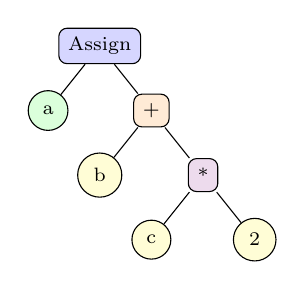
\begin{tikzpicture}[level distance=1.0cm,sibling distance=1.6cm,scale=0.82,every node/.style={font=\scriptsize}]
\node[draw,fill=blue!16,rounded corners=3pt] {Assign}
  child {node[draw,fill=green!14,circle] {a}}
  child {node[draw,fill=orange!16,rounded corners=3pt] {+}
    child {node[draw,fill=yellow!16,circle] {b}}
    child {node[draw,fill=violet!14,rounded corners=3pt] {*}
      child {node[draw,fill=yellow!16,circle] {c}}
      child {node[draw,fill=yellow!16,circle] {2}}}};
\end{tikzpicture}
\end{center}

3AC (one operation per line, temporaries $t_i$):
\begin{align*}
t_1 &= c * 2\\
t_2 &= b + t_1\\
a &= t_2
\end{align*}
Optimised? No change here; constant folding would replace $c*2$ only if $c$ known constant. Register-allocated MIPS (assuming $a,b,c$ in memory):
\begin{lstlisting}[language=C]
# MIPS-like: $t0,$t1 temporaries, $a0 holds &a etc. (illustrative)
lw $t0, b
lw $t1, c
sll $t1, $t1, 1   # c*2 == c <<1  (strength reduction, Ch.6)
add $t0, $t0, $t1
sw $t0, a
\end{lstlisting}
Diagnostics must point at source: if \texttt{c} undeclared, the error at line:col of \texttt{c}, not at \texttt{t1}.

% TikZ 3: correctness as commuting square
\begin{figure}[h]
\centering
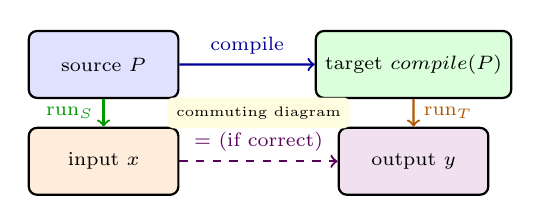
\begin{tikzpicture}[scale=0.82,every node/.style={font=\scriptsize}]
\node[draw,thick,fill=blue!12,minimum width=1.9cm,minimum height=0.85cm,rounded corners=3pt] (src) at (0,1.5) {source $P$};
\node[draw,thick,fill=green!14,minimum width=1.9cm,minimum height=0.85cm,rounded corners=3pt] (tgt) at (4.8,1.5) {target $\text{compile}(P)$};
\node[draw,thick,fill=orange!14,minimum width=1.9cm,minimum height=0.85cm,rounded corners=3pt] (in) at (0,0) {input $x$};
\node[draw,thick,fill=violet!12,minimum width=1.9cm,minimum height=0.85cm,rounded corners=3pt] (out) at (4.8,0) {output $y$};
\draw[->,thick,blue!60!black] (src)--(tgt) node[midway,above] {compile};
\draw[->,thick,green!60!black] (src)--(in) node[midway,left] {run$_S$};
\draw[->,thick,orange!70!black] (tgt)--(out) node[midway,right] {run$_T$};
\draw[->,thick,dashed,violet!70!black] (in)--(out) node[midway,above] {$=$ (if correct)};
\node[font=\tiny,fill=yellow!12,rounded corners=2pt] at (2.4,0.75) {commuting diagram};
\end{tikzpicture}
\caption{Correct compilation: running $P$ on $x$ at source level equals running $\text{compile}(P)$ on $x$ at target level (for defined behaviours). Optimisations must keep the square commuting.}
\label{fig:correctness}
\end{figure}

% ============================================================
\section{Driver, Diagnostics, and Toolchain}
\label{sec:driver}
A \emph{compiler driver} (e.g., \texttt{clang}, \texttt{gcc}) orchestrates: preprocess $\to$ compile $\to$ assemble $\to$ link. It invokes the compiler proper (source$\to$object) then linker (objects+libs$\to$executable). Options select optimisation levels ($-O0$ vs.\ $-O2$), debug info, and warnings.

Diagnostics are not afterthoughts: keep source locations through every IR; emit ``error: use of undeclared identifier 'c' at 3:9'' with a snippet, not ``IR tmp t1 undefined''. Modern compilers store \emph{spans} per node.

\begin{example}[Driver in 20 lines]
\begin{lstlisting}[language=Python]
# Highly simplified driver; real one handles temp files, parallel jobs, caching
def compile_file(src_path, opt_level=2):
    text = open(src_path).read()
    toks = lex(text, filename=src_path)        # Ch.2: LexResult with spans
    ast  = parse(toks)                          # Ch.3: may raise ParseError
    sema(ast)                                   # Ch.4: name/type errors here
    ir   = lower(ast)                           # Ch.5: AST -> 3AC/SSA
    if opt_level >= 1: ir = optimise(ir)        # Ch.6
    asm  = codegen(ir, target="aarch64")        # Ch.7
    obj  = assemble(asm)
    return link([obj], libs=["libc"])
\end{lstlisting}
\end{example}

\subsection*{What can go wrong?}
Formal semantics helps: undefined behaviour (e.g., signed overflow in C) means the commuting square need not hold---the compiler may assume it never happens and optimise accordingly. Phase ordering matters too: constant propagation enables dead-code elimination, but not vice versa.

% ============================================================
\section{Chapter Notes}
Language design and compilation co-evolve: Fortran (1957) invented the compiler; Lisp introduced trees as code; C exposed the machine; Rust makes ownership checkable at compile time. The front/middle/back split matured in LLVM (Lattner, 2004) and GCC. For theory, SC2203's regular/CF languages are the foundation; for practice, Appel's \emph{Modern Compiler Implementation} and Aho--Lam--Sethi--Ullman (\emph{Dragon Book}) are the two complementary bibles---this textbook follows Appel's structure with Dragon-Book rigour.

% ============================================================
\section{Exercises}
\label{sec:ch01-exercises}
\begin{enumerate}[label=E1.\arabic*, leftmargin=*, itemsep=0.8em]
\item \textbf{Phases vs.\ passes.} Give a one-pass design that fuses semantic checking and IR lowering over the AST. What coupling cost does it pay versus two separate passes? Sketch both traversals as visitor pseudocode.
\item \textbf{Token trace.} Lex \texttt{sum = x1\_2 + 0xFF // comment} assuming identifiers \texttt{[a-zA-Z\_][a-zA-Z0-9\_]*}, hex \texttt{0x[0-9a-fA-F]+}, and \texttt{//} line comments. List tokens with lexemes and argue why \texttt{x1\_2} is one token not three.
\item \textbf{AST vs.\ parse tree.} Draw full parse tree and then AST for \texttt{a = b + c * 2} under grammar $E \to E+E \mid E*E \mid \texttt{id}$. Mark dropped nodes and explain why the AST is sufficient for later phases.
\item \textbf{Front/middle/back counting.} With $5$ source languages and $4$ targets, how many compilers without IR vs.\ with one shared IR? If IR is lossy (cannot express one language's feature), what cost appears? Propose a fix.
\item \textbf{Correctness with UB.} C says signed overflow is undefined. Show how \texttt{for(i=0;i<=N;i++) a[i]=0} with \texttt{N==INT\_MAX} can be miscompiled if the compiler assumes \texttt{i+1 > i} always. What does the commuting diagram say?
\end{enumerate}
% End of Chapter 1
